\documentclass[9pt,journal,compsoc]{IEEEtran}
\usepackage[english]{babel}
\usepackage[utf8]{inputenc}
\usepackage{cite}
\usepackage{amsthm}
\usepackage{amsmath}
\usepackage{amssymb}
\usepackage{graphicx}
\usepackage{array}
\usepackage{algorithmic}
\usepackage{url}

% correct bad hyphenation here
\hyphenation{op-tical net-works semi-conduc-tor}

\newtheorem{mydef}{Definition}


\begin{document}

\title{\huge Artificial Neural Networks in Feature Extraction: A Review}

% Author information
\author{
	\IEEEauthorblockN{Joaquim Leitão\IEEEauthorrefmark{1}}
	
	\IEEEauthorblockA{\IEEEauthorrefmark{1}jpleitao@dei.uc.pt \\ CISUC, Department of Informatics Engineering, Univesity of Coimbra, Portugal}
}

% The paper headers
\markboth{Real Time Learning in Intelligent Systems, 2016-2017}{Real Time Learning in Intelligent Systems, 2016-2017}


\IEEEtitleabstractindextext{
\begin{abstract}
	Lol, the abstract
\end{abstract}

\begin{IEEEkeywords}
	Feature Extraction, Artificial Neural Networks.
\end{IEEEkeywords}
}


% make the title area
\maketitle
\IEEEdisplaynontitleabstractindextext
\IEEEpeerreviewmaketitle


\IEEEraisesectionheading{\section{Introduction}\label{sec:introduction}}

\IEEEPARstart{I}{ntro}

Dizer que foco na utilização de redes neuronais para efeitos de feature extraction (nao tanto de selection)

Colocar sigla para Feature Extraction - FE

4 pages

Do not forget to provide an overview of the paper!

\section{Background}\label{sec:background}

The current section addresses the importance of Feature Extraction in Intelligent Systems. In the literature this concept is often presented in the sequel of the well-known curse of dimensionality phenomenon, as a collection of methods that allow a reduction in the problem's dimensionality.

\subsection{Curse of Dimensionality}
\label{curse_dimensionality}

The curse of dimensionality refers to how certain learning algorithms may perform poorly when confronted with high-dimensional data. In many Machine Learning (ML) problems, specially in \emph{classification} tasks, low-dimension feature spaces may not allow for a good separation of the data, leading to low-accuracy classifications. By considering more features, a feature space where an hyperplane that perfectly separates the (training) data can be determined with a resulting increase in classification accuracy.

Nonetheless it has been demonstrated that, as dimensionality increases, the amount of training data needed to accurately generalise the produced classifier grows exponentially. In addition, a small \emph{training samples-to-features} ratio may also degrade performance \cite{jain2000statistical}.

In practice, as training data is limited a scenario similar to figure \ref{curse_dimensionality_fig} is observed: for a given training dataset, classification performance increases as more features are added until an optimum is reached. Further increasing the dimensionality decreases classification performance.

\begin{figure}[ht]
	\centering
	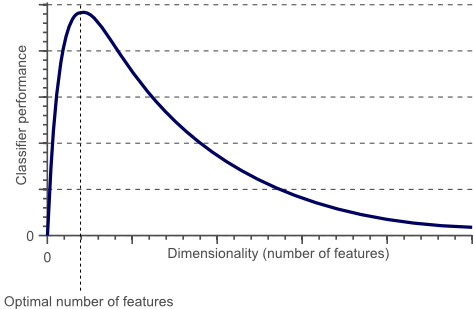
\includegraphics[scale=0.35]{dimensionality_vs_performance.png}
	\caption{Curse of Dimensionality. Taken from \cite{curse_dimensionality_website}.}
	\label{curse_dimensionality_fig}
\end{figure}

A practical implication of the curse of dimensionality is that a system designer should select a small number of features when confronted with a limited training dataset. A general accepted practice is to keep the number of training samples at least ten times higher than the dimensionality: $n / d > 10$ \cite{jain2000statistical}.

\subsection{Dimensionality Reduction}

In light of the discussion conducted in \ref{curse_dimensionality}, a common interest in the vast majority of ML applications is to keep the number of features as small as possible.

Feature Extraction and Feature Selection techniques are the most cited and recognised methods for achieving dimensionality reduction in PR problems. Feature Extraction algorithms propose a new set of features by performing transformations on a given feature set. On their turn, Feature Selection algorithms (ideally) select the best subset of features a provided feature set. As pointed out by Jain \emph{et al.} \cite{jain2000statistical}, feature extraction is typically applied before feature selection\footnote{The idea is to start by defining a new feature set based on the original one, and then select the features that, hopefully, allow a complete separation of the training data.}.

The main issues in dimensionality reduction, namely in feature extraction and selection, are related with the choice of criterion function and the appropriate dimension for the reduced feature space.

\section{Neural Networks in Feature Extraction}\label{sec:anns_feature_extraction}

Artificial Neural Networks (ANNs) have been extensively applied in the field of machine learning, in both classification and regression tasks. Because of their self-learning and trained characteristics, ANNs have also been successfully applied in FE tasks.

Considering the simplest form of ANNs, feedforward networks, FE can be obtained in the output of each hidden layer: the application of the neurons' activation function to the layer's input produces an output that can be interpreted as a set of new features \cite{jain2000statistical}. Depending on the neurons' activation function this new set of features can be a linear or nonlinear combinations of the features in the input feature set (Usually is nonlinear).

It is common to find in the literature types of ANNs where the learning procedure is supervised, and others which perform unsupervised learning. In the task of FE, supervised learning can be difficult to implement, as it requires the correct representation in the low-dimensional space for each training instance.

Instead, ANNs used for FE tend to adapt a different approach: They are trained to reconstruct input samples at the output layer \cite{kramer1992autoassociative}, and in this process ANNs learn an encoder and a decoder, to encode and decode the input sample in a lower dimension space. Again, this can either be linear or nonlinear, depending on the neurons' activation functions (often is nonlinear). Such learning procedure is classified as unsupervised in the literature\cite{fabius2014variational}.

In the remainder of the current section the most popular and referenced ANN architectures applied in FE tasks are intended to be covered. Such architectures include \emph{Feedforward} (namely \emph{Stacked Autoencoders}), \emph{Convolutional}, \emph{Recurrent}, \emph{Radial Basis}, \emph{Restricted Boltzmann Machines} and \emph{Self-Organising Maps}\cite{jain2000statistical, masci2011stacked, kvascev2012radial, fabius2014variational, cho2014learning, marchi2017deep}.

\textbf{FIXME: Rever a lista de arquitecturas para confirmar que não me esqueci de nehuma!!}

\subsection{Feedforward}

In the beginning of the current section feedforward networks were used as a motivation for the application of ANNs in FE tasks.

In its simplest forms, FE can be achieved through single or multi-layer feedforward ANNs by training the network to reconstruct the input signal in a conventional way, using a backpropagation algorithm (or other popular alternatives). Additional layers can also be considered to perform other tasks, such as classification. In this scenario training examples to which the output class is known are fed to the network, and the FE process is learned automatically in the early layers. Networks trained with this approach have been proven to suffer from well-known \emph{vanishing gradient} problems\cite{nielsen2015neural}.

In this sense, training of feedforward networks for FE purposes usually comprises two steps: \emph{Pre-training} and \emph{Fine tuning}.

During pre-training each hidden layer involved in the FE process is trained independently of the others in an unsupervised way: A series of 3-layer feedforward nets are trained to reconstruct their respective inputs at the output layer. The idea is to make each network learn an encoder and a decoder\footnote{The encoder is learned from the input to the hidden layer, while the decoder is learned from the hidden to the output layer.}. In this process, the first network is trained with the input data; the second network is trained with the output of the first network's encoder, and so on. This process is illustrated in figure \ref{barata_saes}.

When pre-training is complete, the encoders are stacked together. Due to this last step, ANNs developed in this way are often referred to as \emph{Stacked autoencoders}.

\begin{figure}[ht]
	\centering
	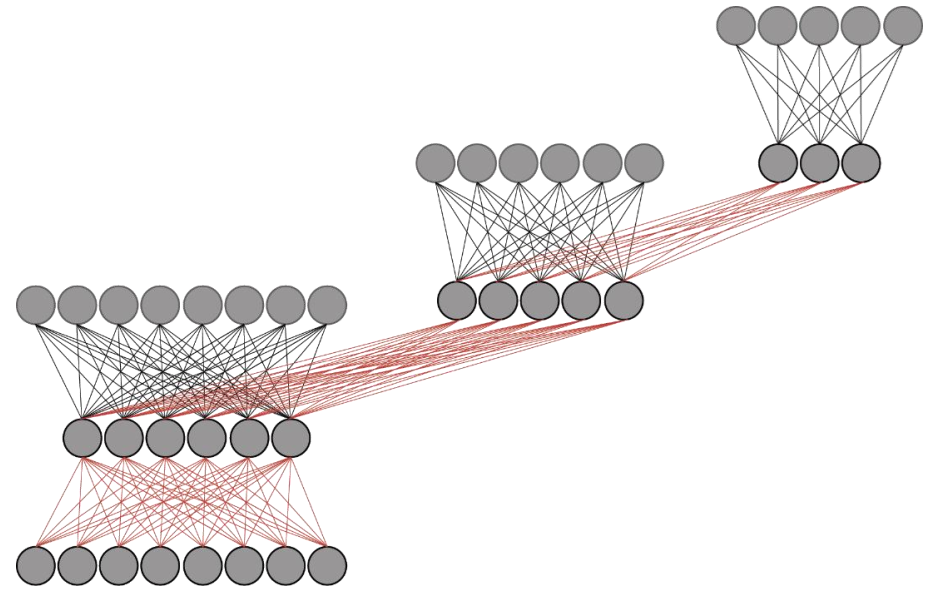
\includegraphics[scale=0.2]{stacked_autoencoders.png}
	\caption{Stacking autoencoders. Taken from \cite{barata_saes_presentation}.}
	\label{barata_saes}
\end{figure}

After the described pre-training, a fine tuning step is usually carried out by considering an additional layer (usually with a softmax activation function) and training the network with backpropagation (or other algorithm), to lightly adjust the weights of the pre-trained layers.

At this moment it is important to address one point in the discussion: based on what has been presented, autoenconders may simply learn the identity function for both the encoder and the decoder, which is not desired. To prevent this, certain activation functions can be forced, producing \emph{regularized autoencoders} such as sparse autoencoders \cite{vincent2010stacked}, denoising autoencoders \cite{ngiam2011optimization} and contractive autoencoders \cite{rifai2011contractive}.

\subsection{Convolutional Neural Networks}



\vspace{5cm}

\subsection{Recurrent Neural Networks}

\subsection{Radial Basis Functions}

\subsection{Restricted Boltzmann Machines}

\subsection{Self-Organising Maps}


\vspace{5cm}

In Self-Organising Maps (SOM), another type of ANN used for NLFE \cite{jain2000statistical, hira2015review}, a low-dimension discretized representation of the input space is produced. Such representation is called a map. A SOM consists of neurons with associated weight vectors (with the same dimension as the input). The neurons are positioned in the map space, usually in a two-dimensional regular spacing in either a hexagonal or rectangular grid (instead of being organised in layers, like in feedforward ANNs).

During the training of a SOM, inputs are presented to the network and, for each, the weight vector closest to the input vector is identified. Then, the weights of all the neurons in the neighbourhood of the winner neuron (that is, the one whose weight vector was selected) are updated, so that they move towards the input vector. In this way, weight vectors of neighbouring neurons in the grid are likely to represent inputs which are close in the original feature space - a "topology-preserving" map is, thus, formed \cite{kohonen1995self, villmann1997topology}. An example of an application where SOM was used for FE can be found in \cite{lawrence1997face}, although many more are available in the literature.

\section{Conclusion}\label{sec:conclusion}

Lol, conclusion

\bibliographystyle{ieeetr}
\bibliography{bibliography.bib}

\end{document}